\titleformat{\chapter}[display]
  {\normalfont\bfseries}{}{0pt}{\Large} % Este comando es para eliminar la aparición de "Capítulo N" en el PDF. Para emplear el formato de la tesis simplemente eliminamos la línea. 
\chapter{Cronograma}
El trabajo de doctorado se organiza de acuerdo con el cronograma de la Figura~\ref{c:1}. En primer lugar, se propone validar las simulaciones de dinámica molecular con los campos de fuerza utilizados en moléculas orgánicas. Luego se pretende calcular la estructura electrónica de los complejos para obtener el de menor energía. Con ello es posible calcular una serie de descriptores cinéticos y realizar un análisis de interacciones por medio de módulos especiales de GROMACS.
\begin{figure}[h]
    \centering
    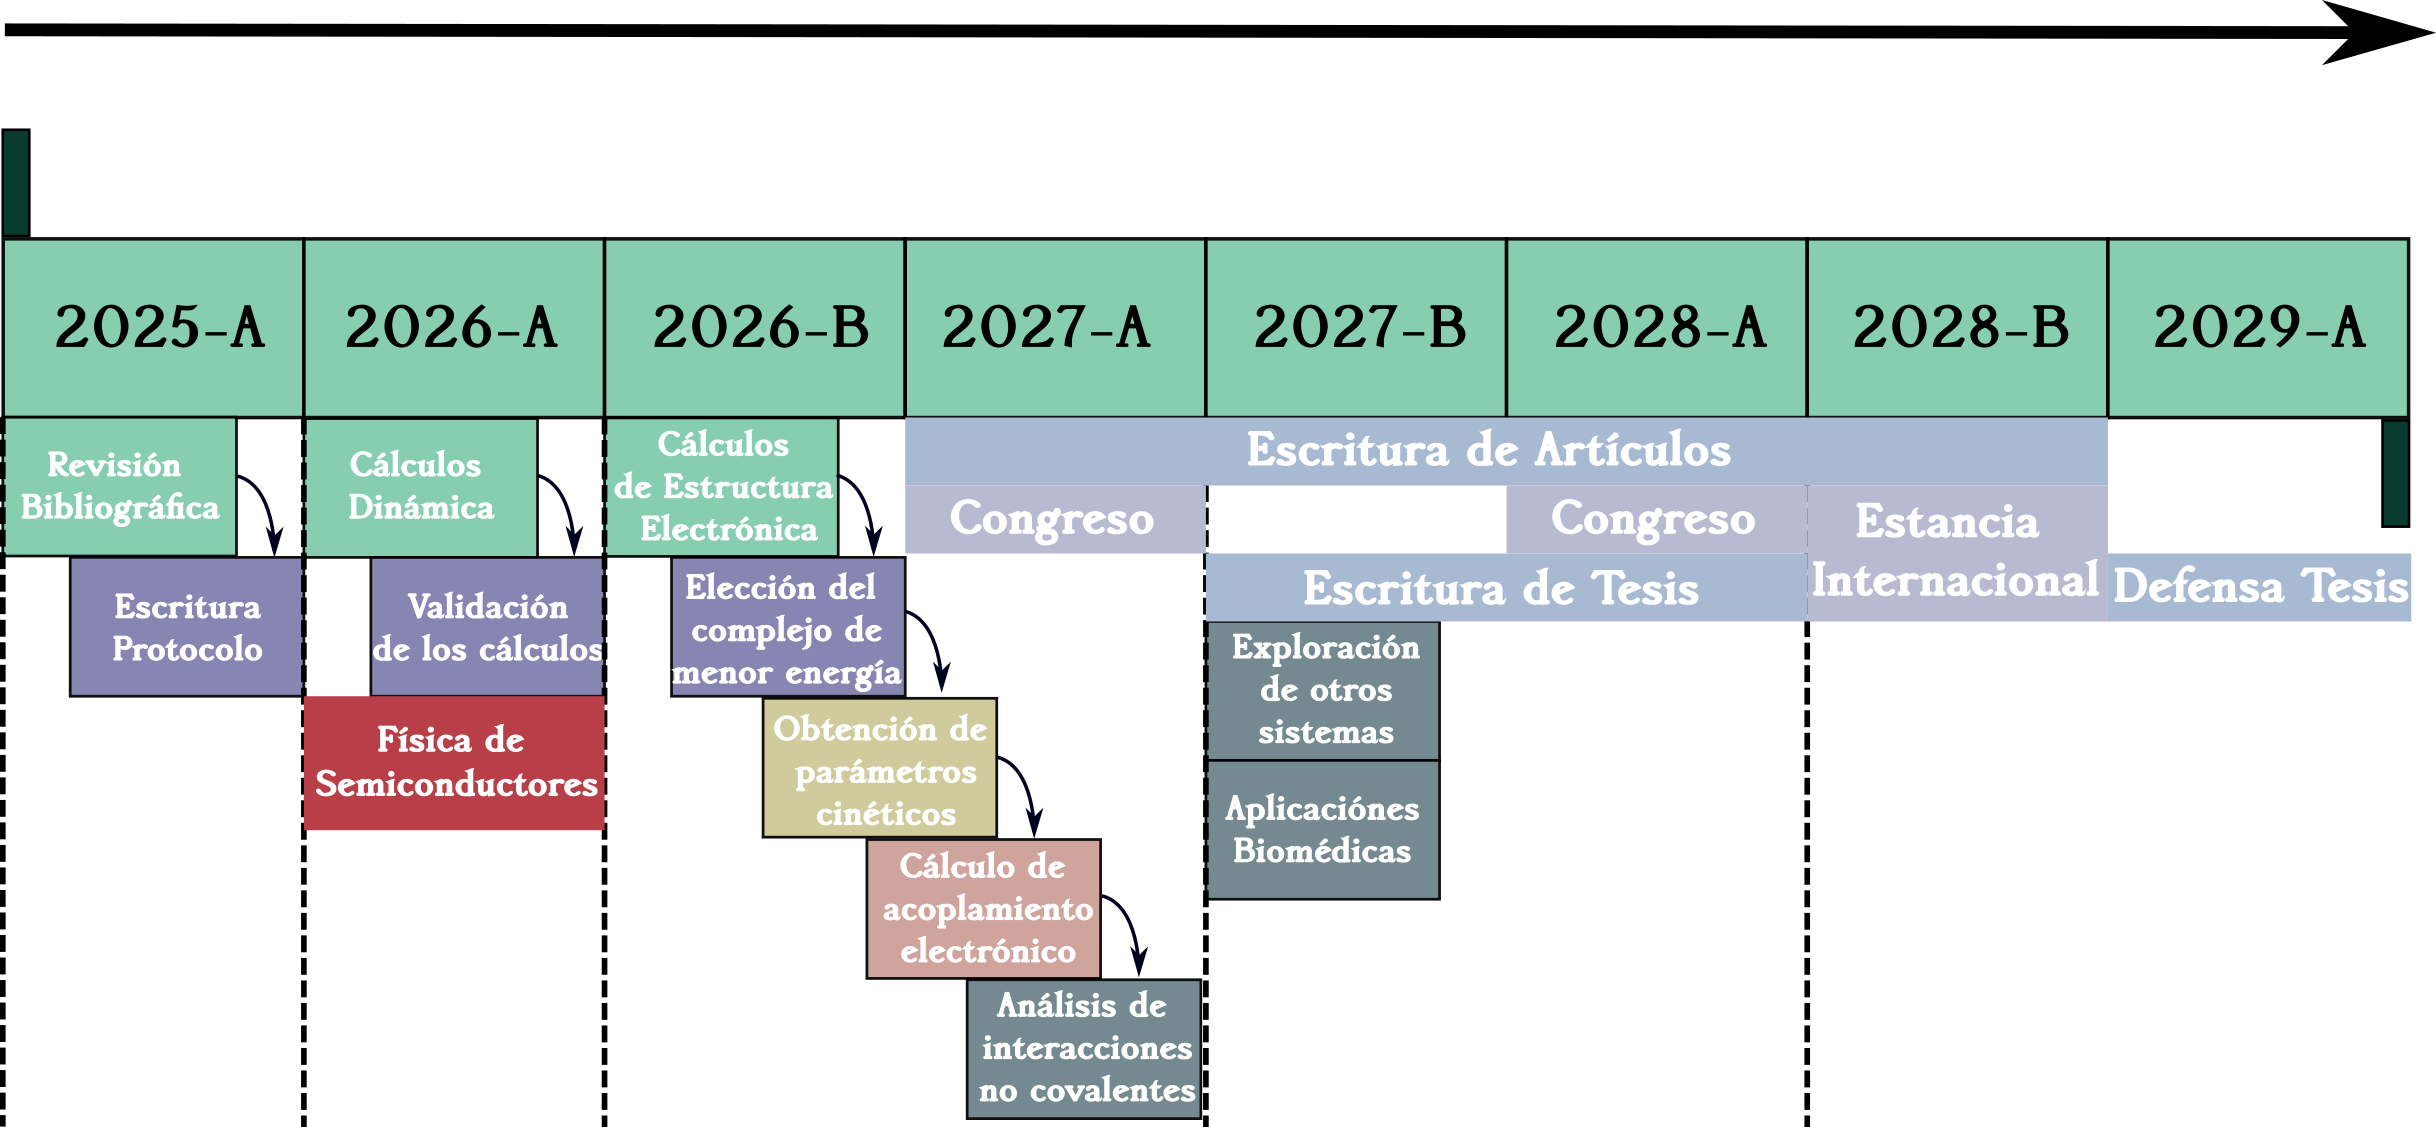
\includegraphics[width=1\textwidth,height=0.5\textwidth]{imagenes/Ant/cro.png}
   \caption{Cronograma de actividades}
    \label{c:1} %Esto genera un numero a mi etiqueta
\end{figure} \\
Finalmente, se contempla redactar dos artículos para su publicación a finales de 2027 o mediados de 2028. También se prevé la participación en dos congresos y una estancia internacional para fortalecer la formación y el conocimiento adquirido durante el doctorado. 